\documentclass[a4paper, 12pt]{article}
\usepackage[T1]{fontenc}
\usepackage[scale=1,angle=0,opacity=1,color=black!60]{background}
\usepackage{tikzpagenodes}
\usepackage{lastpage}
\usepackage{lmodern}
\usepackage{float}
\usepackage[textwidth=420pt,textheight=630pt]{geometry}
\setlength{\oddsidemargin}{15.5pt}
%\usepackage[none]{hyphenat} %no cortar palabras
\usepackage{url}
\usepackage{amsmath}
\usepackage{hyperref}

\usepackage[spanish, activeacute]{babel} %Definir idioma español
\usepackage[utf8]{inputenc} %Codificacion utf-8
\backgroundsetup{contents={}} %Saca el 'draft'

\def\labelitemi{$\bullet$}

\begin{document}
	% TÍTULO, AUTORES Y FECHA
	\begin{titlepage}
		\vspace*{\fill}
		\begin{center}
			\Huge App Server: Definición de Arquitectura \\
			\bigskip\bigskip\bigskip
			
		\end{center}
		\vspace*{\fill}
	\end{titlepage}
	\pagenumbering{arabic}
	\newpage

	% ÍNDICE
	\tableofcontents
	\newpage
	%\pagenumbering{arabic}

	\section{Definición de Arquitectura}
	El app server implementa una API REST utilizada para un sistema de venta de artículos. Esta API es consumida por una app de Android. A su vez se comunica con otro servidor que administra los pagos, envíos y cotización 
	de estos últimos. se puede ver un esquema de comunicación en la siguiente imagen: \\
	
	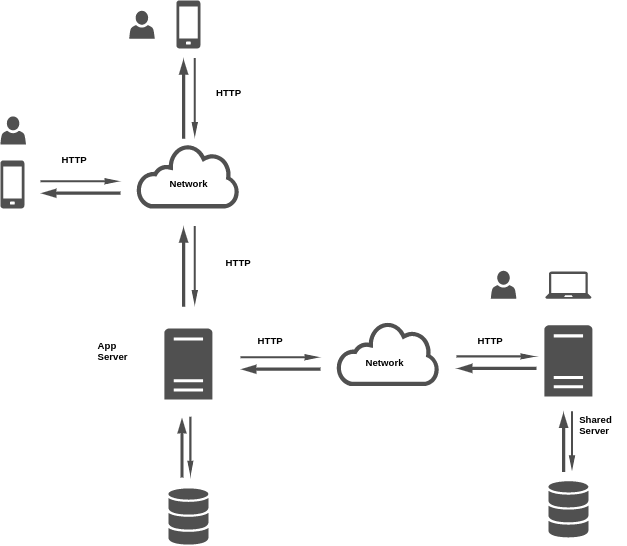
\includegraphics[width=\linewidth]{diagrama.png}
	
	La comunicación entre los dispositivos móviles y el servidor se inicia mediante Google Firebase, una plataforma Backend-as-a-Service (BaaS), mediante el cual provee muchos servicios. Entre estos, se encuentra el servicio de
	 autenticación y el de cloud messaging, que fueron utilizados en este proyecto.
	 
	Para implementar este servidor se utilizó el lenguaje de programación Python y Flask como web framework.Se utilizaron librerías para Flask/Python para realizar la autenticación de los usuarios,
	la serialización y deserialización de los datos y otras librerías comunes para este tipo de desarrollo.
	
	La aplicación inicia ejecutando procesos de configuración del mismo. Luego, antes de empezar a recibir peticiones, se registra en el Shared Server (hay varios App Server que se van a comunicar con un solo Shared Server) 
	y obtiene un id y un token de refresco. Este id y token los guarda en un archivo para utilizarlos a partir de su primera conexión en adelante.
	Una vez que se registró con el shared server empieza a recibir peticiones de los dispositivos móviles. El proceso de registro de estos es el siguiente:
	
	\begin{itemize}
	\item El dispositivo móvil se autentica ante Firebase, obteniendo un token.
	\item El dispositivo móvil se registra entrando al endpoint de registro del app server, obteniendo un id
	\item Con este id y el token de Firebase accede al endpoint de login.
	\item El app server valida ante Firebase que el token sea válido, así como el id.
	\item Se obtiene un token que se utilizará para acceder al resto de los servicios del app server
	\end{itemize}
	
	Para la autenticación del app server se utilizan tokens del tipo JWT.
	
	Se utiliza como base de datos MongoDB, una base de datos no relacional que otorga un modelo de datos flexible. Se utilizó un servicio cloud de MongoDB.
	

	\section{Diseño de aplicación}
	El diseño de la aplicación cuenta con tres capas principales:
	
	\begin{itemize}
	\item Controllers: Es el encargado de proveer el enrutamiento de la aplicación así como recibir las peticiones y preparar las respuestas.
	\item Services: Implementa la lógica de negocio así como las validaciones.
	\item Data: Esta capa se encarga de las consultas e inserciones a la base de dato.
	\end{itemize}
	
	
\end{document}